Using the optimization frameworks developed above, this section evaluates the performance of Shadow Computing by comparing with traditional replication. Without a disparate treatment of the replicas, traditional replication requires all replicas execute at the same rate. In the comparison, however, we also optimize the rate for traditional replication, referred to as optimal traditional replication, in order to demonstrate the benefits of the unique design in Shadow Computing. The following subsections compare between Shadow Computing and state machine replication for crash failure and silent data corruption, respectively. 

\subsection{Comparison for crash failure}
Careful analysis of the models reveal that several parameters, reflective of both the execution environments and the underlying application, affect the behavior of Shadow Computing. These parameters include static power ratio, laxity in deadline and workload. To mimic future extreme-scale environment, the system is set to have $2^{20}$ (~1 million) processors, and each processor has a 5 years' Mean Time Between Failures (MTBF). The impacts of each parameter are shown in Figure~\ref{fig:crash_eval}, with the energy consumption normalized to that of 100 hours of workload.

\begin{figure}[!t]
	\begin{center}
		\subfigure[Impact of static power ratio. $W=24$ hours per processor, $\alpha=25\%$.]
		{
			\label{fig:crash_power}
			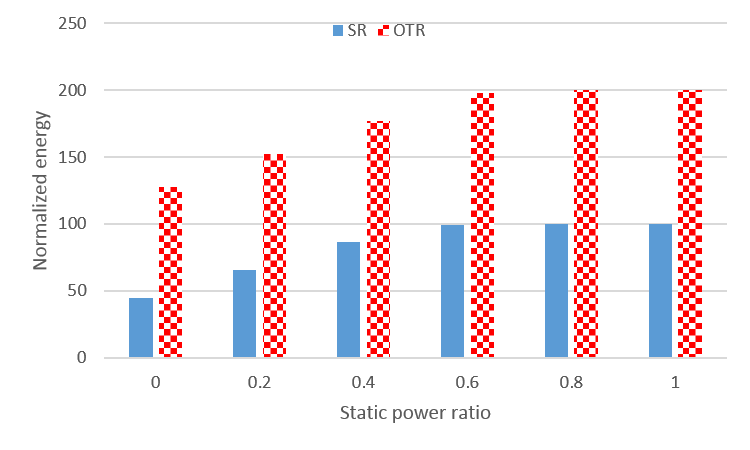
\includegraphics[width=0.4\textwidth]{figures/crash_power}
		}
		\subfigure[Impact of laxity. $W=24$ hours per processor, $\rho=0.3$.]
		{
			\label{fig:crash_laxity}
			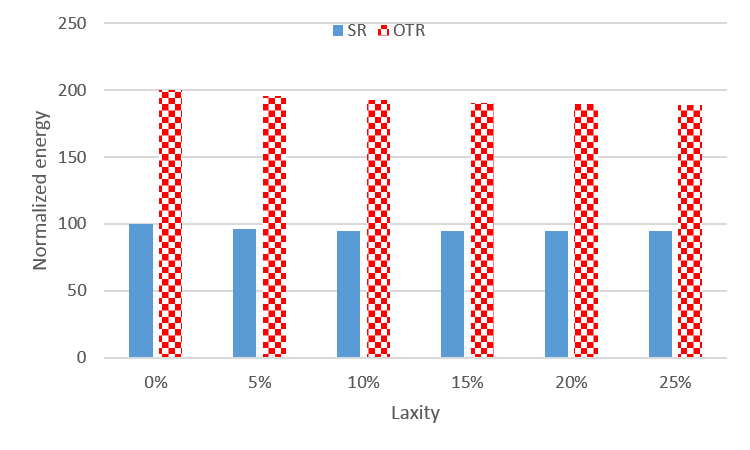
\includegraphics[width=0.4\textwidth]{figures/crash_laxity}
		}
        \subfigure[Impact of workload. $\alpha=25\%$, $\rho=0.5$.]
		{
			\label{fig:crash_workload}
			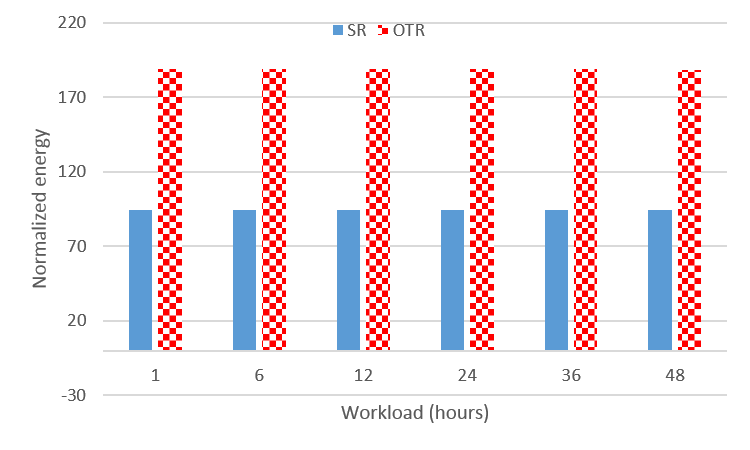
\includegraphics[width=0.4\textwidth]{figures/crash_workload}
		}
	\end{center}
	\caption{Energy comparison between Shadow Computing and Optimal Traditional Replication for under crash failures. $N=2^{20}$, MTBF=5 years.}
	\label{fig:crash_eval}
    \vspace{-0.2in}
\end{figure}

%The static power ratio abstracts the differences in system architecture and organization that impact power consumption. Without considering the deadline, static power ratio determines the optimal execution rate(s) to minimize energy, since it determines the portion of power that is unaffected by the execution rate. However, the optimal rate(s) may not be viable for the consideration of deadline. 
Figure~\ref{fig:crash_power} shows the impact of the static power ratio, ranging from 0 (i.e., no static power) to 1 (i.e., no dynamic power), when there is 25\% laxity in deadline. As we can see, the smaller the static power ratio is, the less energy Shadow Computing and traditional replication consume. This is because they can take advantage of the laxity and slow down. When static power ratio is above 0.8, slowing down does not reduce energy even though there is laxity. 

Between Shadow Computing and optimal traditional replication, the former is able to save more than 49.9\% of energy in all instances, and the saving goes up to 64.9\% when static power ratio is 0. The saving results from the design in Shadow Computing that replicas consume the data partition from two ends. Even with a large number of replica pairs, only a small fraction of them will experience a failure, leaving the majority of partitions processed in a no-redundancy manner. Similarly, differentiating the rates before and after failure allows Shadow Computing to optimize for the most common scenario, i.e., to reduce the rate before failure as much as possible at the cost of increased rate after failure.

Laxity is another important factor that constrains how much Shadow Computing and traditional replication can slow down without missing the deadline. When there is no laxity, both of them have to execute all replicas at the maximum rate, leading to maximum energy. As laxity increases, both approaches will continue to slow down to reduce energy. %, until they reach the optimal rate(s) determined by the static power ratio. 
This is shown in Figure~\ref{fig:crash_laxity}. %Another observation is that laxity has negligible impact on the energy comparison between the two alternatives. Shadow Computing saves around 50\% energy in all cases. 

Given a number of processors, workload determines the execution time, and thus the propensity of the job to failures. For Figure~\ref{fig:crash_workload}, we vary the workload per processor from 1 hour to 2 days. Compared to the 5 years' MTBF, all the workloads considered are relatively small, thus the failure of a given task is very unlikely. Therefore, there is only slight change in the energy consumption. That being said, the impact of workload on the shadowed set level failure is much larger, since each shadowed set consists of multiple pairs of fast and slow replicas. This can be demonstrated by the collocation ratio, which is equal to the number of replica pairs. When workload is 1 hour per processor, 8 slow replicas are allowed to collocate on a processor. With a 48 hours workload, at most 2 slow replicas can collocate. 

\subsection{Comparison for silent data corruption}
Similar to the analysis above, we identify the important parameters of static power ratio, laxity in deadline, workload, number of voting interval, and leaping cost, and study the impact of each one. Again, we fix MTBF to be 5 years for realistic consideration. Also, because workload does not change the energy comparison as in above subsection, we do not show its study and instead fix it to be 100 hours per processor. The comparison results are shown in Figure~\ref{fig:silent_eval}.

\begin{figure*}[!t]
	\begin{center}
		\subfigure[Impact of static power ratio. $\alpha=50\%$, $N=10$.]
		{
			\label{fig:silent_power}
			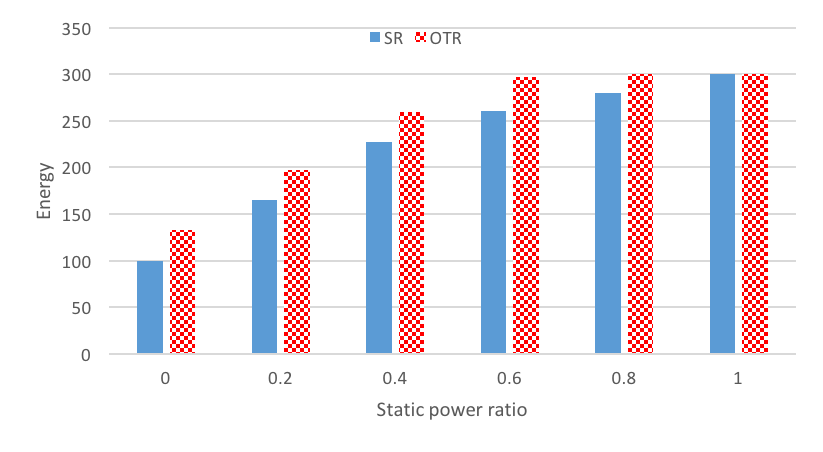
\includegraphics[width=0.4\textwidth]{figures/silent_power}
		}
		\subfigure[Impact of laxity. $\rho=0.3$, $N=10$.]
		{
			\label{fig:silent_laxity}
			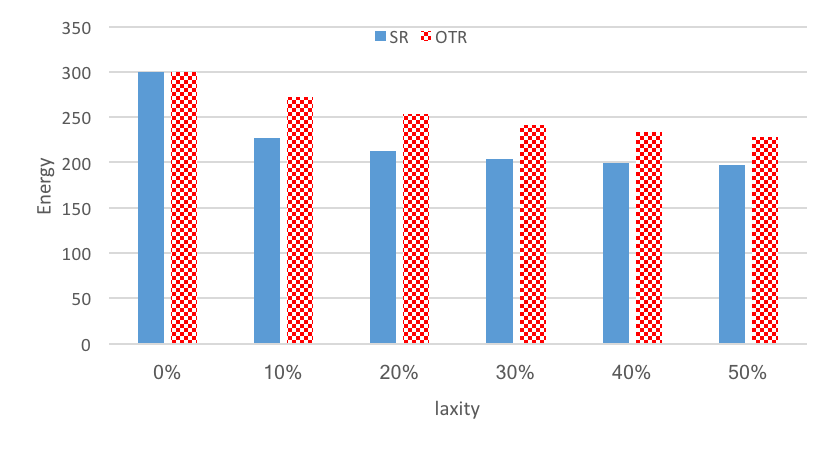
\includegraphics[width=0.4\textwidth]{figures/silent_laxity}
		}
        \subfigure[Impact of voting interval. $\alpha=50\%$, $\rho=0.5$.]
		{
			\label{fig:silent_interval}
			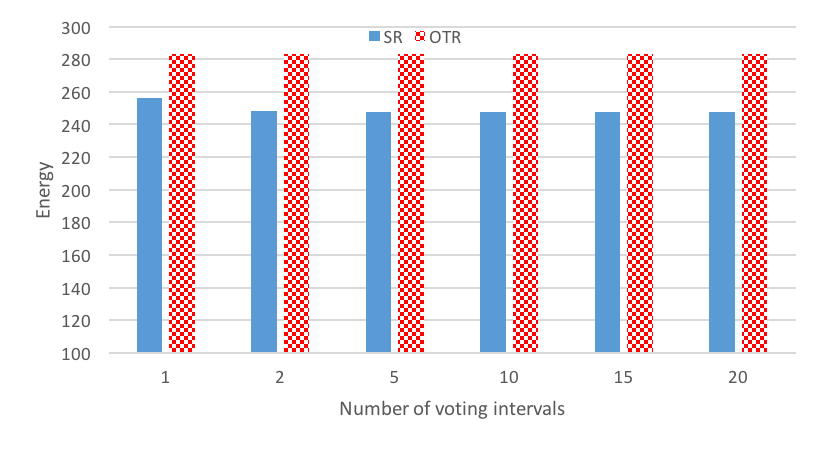
\includegraphics[width=0.4\textwidth]{figures/silent_interval}
		}
        \subfigure[Impact of leaping cost. $\alpha=50\%$, $\rho=0.5$, $N=10$.]
		{
			\label{fig:silent_leap}
			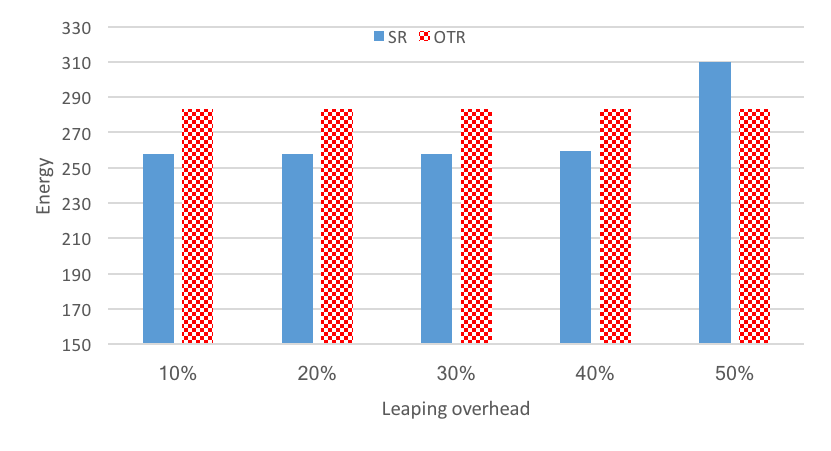
\includegraphics[width=0.4\textwidth]{figures/silent_leap}
		}
	\end{center}
    \vspace{-0.2in}
	\caption{Energy comparison between Shadow Computing and Traditional Replication under silent data corruption. $W=100$ hours, MTBF=5 years.}
	\label{fig:silent_eval}
    \vspace{-0.2in}
\end{figure*}

Figure~\ref{fig:silent_power} reveals the energy consumption of the two compared approaches at different static power ratios, when laxity is 50\% and number of voting intervals is 10. When static power ratio is less than 0.8, both approaches reduces the execution rates to minimize energy. At 0 static power ratio, Shadow Computing saves 25.6\% energy than traditional replication. The saving decreases as static power ratio increases, and finally Shadow Computing converges to traditional replication. Note that energy saving is less than that of crash failure tolerance because both fast and slow replicas have to process a partition from the same end.

With 10 voting intervals and 0.3 as the static power ratio, the impact of laxity is illustrated in Figure~\ref{fig:silent_laxity}. When there is no laxity, Shadow Computing is forced to execute all three replicas at the maximum rate, which is essentially traditional replication. As laxity increases, both approaches have more room to slow down, thereby reducing energy. By coupling two fast replicas with one slow one and uses leaping to achieve forward progress for the slow replica, Shadow Computing always saves 13.5\%-16.9\% energy compared to traditional replication when there is laxity.

One interesting question is how the number of voting intervals change the picture. Without considering the overhead of leaping, intuition tells us that the more voting intervals, the less effect a failure can have, and thus the better performance. This is mostly true, according to Figure~\ref{fig:silent_interval}. However, the figure also shows that after reaching 5, its impact becomes negligible. 

All the above experiments ignore the overhead of leaping. Assuming each time leaping consumes 1 unit of energy, the last experiment studies the impact of leaping overhead, which is defined as a fraction of the workload. Figure~\ref{fig:silent_leap} reveals that when the overhead is below 30\%, it has negligible impact. At 40\% overhead, Shadow Computing slightly increases its rates, and thus incurs a higher energy consumption. When overhead is 50\%, it essentially offsets the laxity, and leaves no room for slowing down. As a result, all replicas need to execute at the maximum rate and end up with consuming more energy than traditional replication.  





